\subsection{Dashboard}\label{dashboard}
Het dashboard is de persoonlijke pagina voor ieder lid van het Intranet. Het is een pagina die is opgebouwd uit blokken die de gebruiker zelf kan aanzetten, uitzetten of verplaatsen.

In de onderstaande afbeelding zie je het Dashboard voor een Intranet gebruiker. 
Bij pijl 1 kun je blokken toevoegen aan je Dashboard. Elk blok heeft verschillende opties zoals inklappen, uitklappen en sluiten. Deze zijn te vinden bij pijl 2.

\begin{center}
	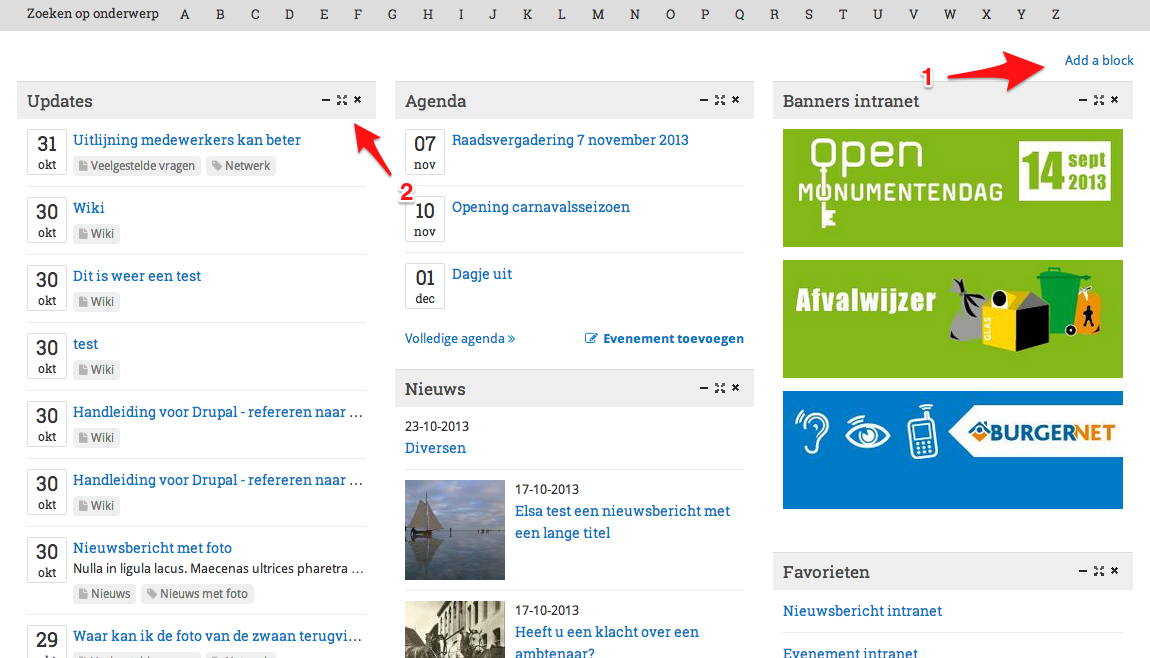
\includegraphics[width=\textwidth]{img/dashboard.png}
\end{center}

\subsubsection{Beheer van blokken}

Als beheerder zijn de mogelijkheden voor gebruikers uit te breiden via \emph{Structuur} $\Rightarrow$ \emph{Homebox} of direct via \drupalpath{admin/structure/homebox}. Daar kan via de link \emph{Lay-out}  een region worden ingesteld voor  bijvoorbeeld het blok "Meeste recente peiling".

